\begin{comment}
\end{comment}

\chapter{Échantillonnage quasi uniforme et comptage approximatif}

\subsection*{Plan}

\begin{enumerate}
    \item Énoncer brièvement l'algorithme de JVV pour introduire la section
    \item Re-mentionner l'importance du comptage approximatif (en autres en comparaison avec le comptage exact)
    \item Mentionner les concepts nécessaires pour l'algorithme de JVV (auto-réductibilité, échantillonnage quasi aléatoire, comptage approximatif)
\end{enumerate}
\subsection*{Références}

%-----------------------------------------------------------------------------%

\section{Auto-réductibilité}
 
\begin{comment}
\subsection*{Plan}

\begin{enumerate}
    \item Introduire les concepts d'auto-réductibilité
\end{enumerate}

\subsection*{Références}

1. Hemaspaandra, L. A. The Power of Self-Reducibility: Selectivity, Information, and Approximation. Preprint at https://doi.org/10.48550/arXiv.1902.08299 (2019).

\subsection*{Brouillon}

Introduction de "Autoreducibility" par Trakhtenbrot.

Introduction de "Self-reducibility" par Schnorr et Meyer/Paterson.

Survey paper de Balcázar, Selke, Allender.

Explication simple par Hemaspaandra.
\end{comment}

L'\textit{auto-réductibilité} ("self-reducibility") est un concept complexe, essentiel à la compréhension du calcul et de la complexité, découlant de l'introduction de la \textit{réduction automatique} (autoreducibility)~\cite{trakhtenbrotAutoreducibility1970}. Ces concepts sont particulièrement importants dans le contexte de génération aléatoire et du comptage approximatif, ainsi que pour la réduction entre le problème de décision et les problèmes de recherche.

La \textit{réduction automatique} peut être introduite informellement de la manière suivante:

\begin{subdefinition}{Réduction automatique}{auto-reductibilite}
    Un problème algorithmique est dit \textit{automatiquement réductible} s'il peut être résolu par un algorithme résolvant d'autres instances du même problème, sans que l'algorithme puisse interroger l'instance particulière qu'il cherche à résoudre.
\end{subdefinition}

Les problèmes automatiquement réductibles contiennent de l'information d'appartenance redondante, c'est-à-dire qu'il existe une structure dans l'ensemble de problèmes pouvant être exploitée pour simplifier le calcul d'une instance donnée. Ainsi, un algorithme peut résoudre une instance en utilisant l'information redondante présente dans d'autres instances, évitant ainsi les requêtes directes à l'instance en question. Connaître la solution à une autre problème peut alors aider la résolution du problème initial. 

\textcolor{mydarkred}{\textit{Exemple: Halting problem?}}

Pour discuter de la génération aléatoire et le comptage approximatif, l'\textit{auto-réductibilité descendante}, une forme limité de la réduction automatique, est une définition plus adéquate. En effet, cette condition est nécessaire à l'application de l'algorithme JVV. Informellement, on peut définir celle-ci comme:

\begin{maindefinition}{Auto-réductibilité descendante}{auto-reductibilite-informel}
    Un problème algorithmique est dit \textit{auto-réductible descendant} s'il peut être résolu grâce à un algorithme résolvant des instances de taille strictement inférieure.
\end{maindefinition}

\textcolor{mydarkred}{\textit{Quelle est vraiment la différence entre auto-reducibility et self-reducibility?}}

Cette propriété s'éclaircit en prenant le problème SAT comme exemple, qui s'avéra particulièrement utile dans la compréhension de l'algorithme JVV à la section~\ref{sec:algorithme-jvv}. L'auto-réductibilité appliquée au problème de satisfaisabilité s'exprime facilement avec la relation suivante:

\begin{relation}{Auto-réductibilité pour les problèmes SAT}{auto-reductibilite-sat}
    Soit une constante $n \geq 1$ et une formule propositionelle $\varphi(x_{1}, x_{2}, \dots, x_{n})$ où $x_{i} \in \set{ 0, 1 }$. Alors,
    \begin{equation*}
        \varphi(x_{1}, x_{2}, \dots, x_{n}) = 1 \iff \varphi(x_{1}=0, x_{2}, \dots, x_{n}) = 1 \lor \varphi(x_{1}=1, x_{2}, \dots, x_{n}) = 1
    \end{equation*}
\end{relation}

Cette relation implique que l'ensemble de solutions d'une instance donnée peut être exprimée comme l'ensemble de solutions de deux instances plus petite du problème. \textcolor{mydarkred}{\textit{Élaborer...}}

Plus précisément, le problème SAT est décrit comme une auto-réductibilité à longueur décroissante 2-disjonctive. Ici, 2-disjonctive fait référence à une formule propositionnelle dans une disjonction ($\lor$) d'une conjonction ($\land$) d'au plus deux variables. Longueur décroissante, ou descendante, signifie que l'algorithme résout des instances de taille strictement inférieure.

Une définition rigoureuse de l'auto-réductibilité peut aussi être pratique.

\begin{maindefinition}{Auto-réductibilité descendante}{auto-reductibilite-formel}
    Soit $\Sigma^{*}$ un ensemble fixé et fini encodant les instances d'un problème ainsi que leurs solutions. Soit $R \subseteq \Sigma^{*} \times \Sigma^{*}$ une relation binaire assignant à chaque instance de problème $x \in \Sigma^{*}$ un ensemble de solutions $R(x) = \set{ y \in \Sigma^{*} \mid xRy }$. Une relation $R \subseteq \Sigma^{*} \times \Sigma^{*}$ est auto-réductible si et seulement si
    \begin{enumerate}
        \item il existe une fonction calculable en temps polynomial $g \in \sigma^{*} \to \mathbb{N}$ tel que $xRy \implies \lvert y \rvert = g(x)$;
        \item il existe une fonction calculable en temps polynomial $\psi \in \Sigma^{*} \times \Sigma^{*} \to \Sigma^{*}$ et $\sigma \in \Sigma^{*} \to \mathbb{N}$ satifaisant
        \begin{align*}
            & \sigma(x)=O(\log |x|) \\
            & g(x)>0 \Rightarrow \sigma(x)>0 \quad \forall x \in \Sigma^{\star} \\
            & |\psi(x, w)| \leqslant|x| \quad \forall x, w \in \Sigma^{\star}
        \end{align*}
        et tel que, pour tout $x \in \Sigma^{*}, y=y_1 \ldots y_n \in \Sigma^{*}$, 
        \begin{equation*}
            \left\langle x, y_1 \ldots y_n \right\rangle \in R \Leftrightarrow \left\langle \psi \left( x, y_1 \ldots, y_{\sigma(x)} \right), y_{\sigma(x)+1} \ldots y_n \right\rangle \in R
        \end{equation*}
    \end{enumerate}
\end{maindefinition}

\textcolor{mydarkred}{\textit{Parler du lien avec les problème de recherche.}}


%-----------------------------------------------------------------------------%

\section{Échantillonnage quasi uniforme}

\begin{comment}
\subsection*{Plan}

\begin{enumerate}
    \item Introduire les FPAUS
    \item Introduire la distance en variation totale et la non-uniformité
\end{enumerate}

\subsection*{Références}
\end{comment}

\begin{maindefinition}{Échantillonneur quasi uniforme pleinement polynomial (FPAUS)}{fpaus}
    Un échantillonneur quasi uniforme pour un ensemble de solutions $S \subseteq \Sigma^{*} \times \Sigma^{*}$, où $S$ représente la relation entre les instances d'un problème $x$ et de ses solutions $y \in  S(x)$, est un algorithme aléatoire prenant en entrée une instance $x \in \Sigma^{*}$ et une tolérance d'échantillonnage $\delta > 0$ et qui génère une solution $y \in S(x)$ tel que
    \begin{equation*}
        \lVert Y - U \rvert_{TV} \leq \delta 
    \end{equation*}
    où $Y$ est la distribution de probabilité de $y$ et $U$ est la distribution de probabilité uniforme sur $S(x)$. Si l'algorithme s'exécute en temps borné par un polynomial en $\lvert x \rvert$ et en $\ln (\delta^{-1})$, on parle d'échantillonneur quasi uniforme pleinement polynomial.
\end{maindefinition}

\textcolor{mydarkred}{\textit{Changer la définition pour celle du papier de JVV? Oui, et décrire le lien avec la TVD.}}

%-----------------------------------------------------------------------------%

\section{Comptage approximatif}

\begin{comment}
\subsection*{Plan}

\begin{enumerate}
    \item Introduire les FPRAS
    \item Introduire les algorithmes de comptage classique connus (ex.: Stockmeyer et JVV)
\end{enumerate}

\subsection*{Références}

1. Stockmeyer, L. The complexity of approximate counting. in Proceedings of the fifteenth annual ACM symposium on Theory of computing 118–126 (Association for Computing Machinery, New York, NY, USA, 1983). doi:10.1145/800061.808740.
\end{comment}

\begin{maindefinition}{Schéma d'approximation aléatoire pleinement polynomial (FPRAS)}{fpras}
    Un schéma d'approximation aléatoire pour un problème de comptage $f: \Sigma^{*} \to \mathbb{N}$ est un algorithme aléatoire prenant en entrée une instance d'un problème $x \in \Sigma^{*}$ et une tolérance d'erreur $\varepsilon > 0$ et qui génère un nombre $N \in \mathbb{N}$ tel que, pour toute instance $x$,
    \begin{equation*}
        \mathrm{ Pr }\left[(1+\varepsilon)^{-1} f(x) \leq N \leq (1+\varepsilon)f(x)\right] \geq \frac{3}{4} .
    \end{equation*}
    Si l'algorithme s'exécute en temps borné par un polynomial en $\lvert x \rvert$ et $\varphi^{-1}$, alors on parle de schéma d'approximation aléatoire pleinement polynomial.
\end{maindefinition}

%-----------------------------------------------------------------------------%

\section{Algorithme de Jerrum-Valiant-Vazirani}
\label{sec:algorithme-jvv}

\begin{comment}
\subsection*{Plan}

\begin{enumerate}
    \item Introduire le but de l'algorithme de JVV
    \item Vulgariser l'algorithme de JVV
    \item Introduire rigoureusement l'algorithme de JVV
    \item Rajouter l'algorithme complet sous forme de pseudo-code.
\end{enumerate}

\subsection*{Références}

1. Jerrum, M. R., Valiant, L. G. and Vazirani, V. V. Random generation of combinatorial structures from a uniform distribution. Theoretical Computer Science 43, 169–188 (1986).
2. Huber, M. Exact sampling and approximate counting techniques. in Proceedings of the thirtieth annual ACM symposium on Theory of computing 31–40 (Association for Computing Machinery, New York, NY, USA, 1998). doi:10.1145/276698.276709.
\end{comment}

\begin{figure}[h]
    \centering
    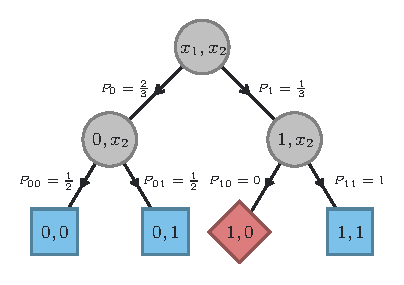
\includegraphics[width=0.5\textwidth]{figures/jvv-algorithm.pdf}
    \caption{}
    \label{fig:jvv-algorithm}
\end{figure}